\documentclass[11pt]{article}

\usepackage{listings}
\usepackage{color}

\definecolor{dkgreen}{rgb}{0,0.6,0}
\definecolor{gray}{rgb}{0.5,0.5,0.5}
\definecolor{mauve}{rgb}{0.58,0,0.82}

\definecolor{mygreen}{rgb}{0,0.6,0}
\definecolor{mygray}{rgb}{0.5,0.5,0.5}
\definecolor{mymauve}{rgb}{0.58,0,0.82}

\lstset{ %
  backgroundcolor=\color{white},   % choose the background color; you must add \usepackage{color} or \usepackage{xcolor}; should come as last argument
  basicstyle=\footnotesize,        % the size of the fonts that are used for the code
  breakatwhitespace=false,         % sets if automatic breaks should only happen at whitespace
  breaklines=true,                 % sets automatic line breaking
  frame=tb,
  captionpos=b,                    % sets the caption-position to bottom
  commentstyle=\color{mygreen},    % comment style
  deletekeywords={...},            % if you want to delete keywords from the given language
  escapeinside={\%*}{*)},          % if you want to add LaTeX within your code
  extendedchars=true,              % lets you use non-ASCII characters; for 8-bits encodings only, does not work with UTF-8
  keepspaces=true,                 % keeps spaces in text, useful for keeping indentation of code (possibly needs columns=flexible)
  keywordstyle=\color{blue},       % keyword style
  language=Octave,                 % the language of the code
  morekeywords={*,...},           % if you want to add more keywords to the set
  numbers=left,                    % where to put the line-numbers; possible values are (none, left, right)
  numbersep=5pt,                   % how far the line-numbers are from the code
  numberstyle=\tiny\color{mygray}, % the style that is used for the line-numbers
  rulecolor=\color{black},         % if not set, the frame-color may be changed on line-breaks within not-black text (e.g. comments (green here))
  showspaces=false,                % show spaces everywhere adding particular underscores; it overrides 'showstringspaces'
  showstringspaces=false,          % underline spaces within strings only
  showtabs=false,                  % show tabs within strings adding particular underscores
  stepnumber=1,                    % the step between two line-numbers. If it's 1, each line will be numbered
  stringstyle=\color{mymauve},     % string literal style
  tabsize=2,                       % sets default tabsize to 2 spaces
}

\renewcommand{\lstlistingname}{Quadro}

\usepackage{color}
\definecolor{lightgray}{rgb}{.9,.9,.9}
\definecolor{darkgray}{rgb}{.4,.4,.4}
\definecolor{purple}{rgb}{0.65, 0.12, 0.82}
\lstdefinelanguage{JavaScript}{
  keywords={break, case, catch, continue, debugger, default, delete, do, else, false, finally, for, function, if, in, instanceof, new, null, return, switch, this, throw, true, try, typeof, var, const, void, while, with},
  morecomment=[l]{//},
  morecomment=[s]{/*}{*/},
  morestring=[b]',
  morestring=[b]",
  ndkeywords={class, export, boolean, throw, implements, import, this},
  keywordstyle=\color{blue}\bfseries,
  ndkeywordstyle=\color{darkgray}\bfseries,
  identifierstyle=\color{black},
  commentstyle=\color{purple}\ttfamily,
  stringstyle=\color{red}\ttfamily,
  sensitive=true
}

\usepackage{enumitem,amssymb}
\newlist{todolist}{itemize}{2}
\setlist[todolist]{label=$\square$}
\usepackage{pifont}
\newcommand{\cmark}{\ding{51}}%
\newcommand{\xmark}{\ding{55}}%
\newcommand{\done}{\rlap{$\square$}{\raisebox{2pt}{\large\hspace{1pt}\cmark}}%
\hspace{-2.5pt}}
\newcommand{\wontfix}{\rlap{$\square$}{\large\hspace{1pt}\xmark}}


\usepackage{environ}
\NewEnviron{todobox}{
\noindent
\shadowbox{%
\begin{minipage}{\dimexpr\textwidth-\shadowsize-2\fboxrule-2\fboxsep}
\textcolor{red}{\sffamily TODO:}\par\vspace{\baselineskip}
\BODY
\vspace{0.05cm}
\end{minipage}}
}
% Fonte em portgues brasileiro
\usepackage[brazilian]{babel}
\usepackage[utf8]{inputenc}
\usepackage[T1]{fontenc}
\usepackage{lmodern}

%%%%%%%%%%Packages opcionais%%%%%%%%%%%%%%

% Tabelas
\usepackage{booktabs}
\usepackage{multirow}
\usepackage{multicol}
\usepackage{tabularx}

% Identação e espaçamento
\usepackage{fullpage}      % Autoscale da página
\usepackage{indentfirst}   % Identar parágrafo em cada quebra de linha

% Figuras
\usepackage{graphicx}      % Pictures
\graphicspath{{./logo/}{./figuras/}} % Pastas para procurar imagens

% URLs na bibliografia
\usepackage{url}
\usepackage{hyperref}
\hypersetup{
    colorlinks,
    citecolor=black,
    filecolor=black,
    linkcolor=black,
    urlcolor=black
}

% não lembro mais
\usepackage{fancybox}


\begin{document}


%---------------------------------------------------
%Começo da capa
\begin{center}
\thispagestyle{empty}

\includegraphics[width=0.1\linewidth]{UFSC} \\[0.3cm]
\textsc{\LARGE Universidade Federal de Santa Catarina}\\[4cm]

\textsc{\large Relatório e Documentação de Desenvolvimento de Projeto}\\[0.5cm]
% Título
\hrule \vspace{0.4cm}
{ \huge \bfseries Monitoramento e Acesso de Portas UFSC Blumenau  \\[0.4cm] }
\hrule \vspace{1.5cm}
\vspace{5cm} % Valor opcional, pode ser definido para alterar a altura dos nomes na página

% Autores e professor
\begin{minipage}{0.5\textwidth}
\begin{flushleft} \large

\end{flushleft}
\end{minipage}
\begin{minipage}{0.4\textwidth}
\begin{flushright} \large
Brunno Vanelli
\end{flushright}
\end{minipage}

\vfill

% Fim da capa
{\large Blumenau \\[0.4cm] Junho de 2017}

\end{center}
% Fim da capa
%---------------------------------------------------



%---------------------------------------------------
%Começo do Sumário
\newpage
% Gerar sumário. É necessário mais de uma compilação para ser gerado completamente.
\tableofcontents
\newpage
% Fim do sumário
%---------------------------------------------------


\section{Introdução}

\subsection{Instalando o toolchain do EPOS}

Para instalar as dependências necessárias e o toolchain do EPOS basta executar o seguinte script, substituindo o usuário correspondente para o repositório do SVN.

\lstinputlisting[language=bash, caption=Script de Instalação do toolchain do EPOS.]{code/eposinstall.sh}

\subsection{Traits}

O EPOS utiliza um arquivo traits para moldar como o sistema vai se comportar e quais módulos serão utilizados. Os traits importantes são:

\lstinputlisting[language=c++, caption=Traits da arquitetura., firstline=18,lastline=34]{code/mfrc522reader_traits.h}
\lstinputlisting[language=c++, caption=Traits do debug USB., firstline=83,lastline=91]{code/mfrc522reader_traits.h}
\lstinputlisting[language=c++, caption=Traits do Hydro Board., firstline=218,lastline=230]{code/mfrc522reader_traits.h}
\lstinputlisting[language=c++, caption=Traits do módulo MFRC522., firstline=237,lastline=241]{code/mfrc522reader_traits.h}

\section{Documentação dos Componentes}

\subsection{MIFARE RFID-RC522}

Leitor RFID para cartões MIFARE ISO/IEC 14443 Tipo A 13.56 MHz. Esse tipo de cartão apresenta armazenamento interno de 1KB e uma chave de 48 bits (padrão \texttt{0xFFFFFFFFFFFF}). O armazenamento interno se parece algo como o Quadro \ref{q:memory}. O protocolo de comunicação com Arduino é o SPI, que necessita de 3 pinos: o \textbf{SCK}, \textbf{MISO} e \textbf{MOSI}. Deve-se conectar também o \textbf{3.3V}, o \textbf{GND} e os pinos \textbf{RST} e \textbf{SDA} (SS).

\begin{center}
\scalebox{.8}{\lstinputlisting[label=q:memory,caption=Bloco de Memória interno dos cartões MIFARE.]{code/mifare.mem}}
\end{center}

A pinagem para conexão do módulo RFID ao Epos Mote III utilizada, seguindo a implementação \texttt{config\_SSI} descrita em \texttt{include/machine/cortex/emote3.h} foi:

\begin{itemize}
\item 3.3V ligado ao 3.3V
\item RST ligado à porta PC6
\item GND ligado ao GND
\item MISO ligado a PA4
\item MOSI ligado ao PA5
\item SCK ligado a PA2
\item SDA ligado à porta PB5
\end{itemize}


\begin{todobox}
\begin{todolist}
\item[\done] Resolver problema de o EPOS ser capaz de reconhecer as portas e inicializar o RFID\_Reader, mas não faz a leitura dos cartões, que foi testado no Arduino.
\item[\done] Testar as portas e comunicação SPI do EPOS no osciloscópio.
\item[\done] Testar novamente o MFRC522 com o osciloscópio.
\item Criar interface RJ45 para conexão do módulo ao eMoteIII.
\item[\done] Criar esquemáticos das ligações.
\end{todolist}
\end{todobox}

\subsection{Hydro Board}

O módulo é do tipo shield e as interconexões são respectivamente, seguindo as especificações em \texttt{src/machine/cortex/hydro\_board\_init.cc}. O acionamento dos relés pode ser alterando o nível lógico nas portas via GPIO ou utilizando a biblioteca.

\begin{itemize}
\item Relé P3 ligado à porta PB0
\item Relé P4 ligado à porta PB1
\item Relé P5 ligado à porta PB2
\end{itemize}

\begin{todobox}
\begin{todolist}
\item Conseguir fonte de tensão regulável ou 12V para o módulo.
\end{todolist}
\end{todobox}

\subsection{ESP8266}

O módulo ESP8266 utiliza comunicação UART para intermediar o eMoteIII e o servidor. As conexões necessárias para comunicação são RX e TX. As portas são:

\begin{itemize}
\item RX do ESP8266 ligado à porta PA1.
\item TX do ESP8266 ligado à porta PA0.
\item Vin e CH do ESP8266 ligado à uma fonte externa de tensão 3.3V (da Hydro Board).
\item Todos os GNDs compartilhados.
\end{itemize}

\begin{todobox}
\begin{todolist}
\item[\done] Reescrever ou fazer funcionar o código ESP8266 do Lisha.
\item[\done] Criar regulador de tensão 3.3V para alimentação da ESP8266.
\item[\done] Criar esquemáticos das ligações.
\end{todolist}
\end{todobox}

\section{Camada de Nuvem}

\subsection{Banco de dados}

O banco de dados utilizado setado para testes e armazenamento foi o Cassandra, utilizado com um driver para NodeJS. Para instalar localmente, basta:

\lstinputlisting[language=bash, caption=Script de Instalação do Cassandra., firstline=1, lastline=5]{code/phpcassandra.sh}

\subsection{Servidor de Acesso}

\begin{todobox}
\begin{todolist}
\item Conseguir um servidor permanente.
\item Fazer deployment de um cluster Cassandra em nuvem.
\item[\done] Instalar versão local no LABCOP.
\item[\done] Implementar segurança.
\end{todolist}
\end{todobox}

\subsection{Modelagem inicial do Banco de dados}

Para modelar o banco de dados, pode-se usar a linha de comando ou usar algum software para gerenciar o banco. Foi utilizado o DBeaver 4.0.5 EE, que não possui versão comercial e está disponível no link \url{https://dbeaver.jkiss.org/files/4.0.5/dbeaver-ee_4.0.5_amd64.deb}.

Para criar uma tabela de acessos no Cassandra, foi utilizado um Keyspace utilizando o comando:

\begin{lstlisting}
CREATE KEYSPACE dados 
	WITH replication = { 'class': 'SimpleStrategy', 'replication_factor': '1' }
\end{lstlisting}

Cada nodo deve ter um \texttt{nodeid} para facilitar a identificação. Esse node ID será introduzido no arquivo de configuração e deve ser único para nodo. Assim, uma tabela para armazenas as relações nodo/sala será:

\begin{lstlisting}
CREATE TABLE IF NOT EXISTS dados.salas_por_nodeid ( 
  updated timestamp,
  sala text,
  id text,
  access_token text,
  PRIMARY KEY (id, access_token)
);
\end{lstlisting}


Então, uma vez que se obtém a sala do nodo através da autenticação, acessa-se a tabela para armazenar as entradas de dados com os UIDs dos cartões magnéticos:

\begin{lstlisting}
CREATE TABLE IF NOT EXISTS dados.uid_por_salas ( 
  updated timestamp,
  sala text,
  uid bigint,
  PRIMARY key (sala, uid)
);
\end{lstlisting}

Para armazenar as relações salas/UIDs, utilizar-se-á uma tabela com esse propósito. Como 'sala' é o PartitionKey, ela indexará a tabela para que as buscas por uma determinada sala sejam facilitadas.

Por fim, como log dos acessos às salas, uma tabela de controle de acesso indexada nos timestamps.

\begin{lstlisting}
CREATE TABLE IF NOT EXISTS dados.log_acesso ( 
  timestamp timestamp,
  uid bigint,
  status_code int,
  id text,
  sala text,
  PRIMARY key ((uid), timestamp)
)
WITH CLUSTERING ORDER BY (timestamp DESC);
\end{lstlisting}

Além do cadastro dos usuários para os sistemas de recursos humanos:

\begin{lstlisting}
CREATE TABLE IF NOT EXISTS dados.usuario_por_uid ( 
  updated timestamp,
  nome text,
  matricula text,
  uid bigint,
  PRIMARY key (matricula)
);
\end{lstlisting}

\begin{todobox}
\begin{todolist}
\item[\done] Criar modelo de banco de dados.
\item[\done] Conversar com o Alex sobre os modelos de tabelas.
\item Otimizar tabelas para satisfazer boas práticas: \url{https://www.datastax.com/dev/blog/basic-rules-of-cassandra-data-modeling}
\item[\done] Criar tipo de dado UID no Cassandra (resolvido com 64 bits signed integer).
\end{todolist}
\end{todobox}



\subsection{Métodos de Acesso}

\subsubsection{Servidor REST}

Foi criado um servidor REST escrito em NodeJS para processar as requisições dos dispositivos e responder adequadamente, guardando os dados de log no banco de dados. A escolha do NodeJS foi devido ao fato de o PHP se mostrar difícil de instalar bibliotecas como o driver Cassandra. Como o Nodejs possui um gerenciador de pacotes e é rápido e escalável, optou-se por utilizá-lo. Para inicializar o servidor, basta:

\begin{lstlisting}
cd rest-api/
npm install
npm start
\end{lstlisting}

\subsubsection{Autenticação}

A autenticação é realizada através do fornecimento de um par ID/token. O ID foi definido e é validado como um valor hexadecimal de 8 caracteres, em formato string, permitindo 4294967296 (4 bilhões) de nodos diferentes, com o conjunto de caracteres [0-9a-f]. O valor do token é definido como uma sequência em base 64, com o conjunto de caracteres [0-9a-zA-Z\_-]. Toda a comunicação é encriptada do servidor ao ESP8266 por meio de SSL.

\lstinputlisting[language=Javascript, caption=Autenticação., firstline=49,lastline=63]{../rest-api/server.js}

\subsubsection{Acesso por GET}

As informações de acesso são armazenadas no banco de dados. O nodo ESP8266 deve então fazer uma requisição para o servidor Apache com o parâmetro salas e seu token de acesso. Para proteger o token de acesso, além da criptografia, é importante utilizar um esquema de desafio, que ainda não foi implementado:

\lstinputlisting[language=Javascript, caption=Caminho do método GET., firstline=70,lastline=98]{../rest-api/server.js}

Pode-se testar a aplicação com curl:

\begin{lstlisting}
curl -k "https://localhost/api/v1/abcdefgh/00000000000000000000"
\end{lstlisting}

Ou por meio das bibliotecas desenvolvidas no EPOS para acesso ao ESP8266:

\begin{lstlisting}[language=C++]
ESP8266 esp8266;
char data[1500];
char * url = "localhost/api/v1/abcdefgh/00000000000000000000";
esp8266.get(url, data, sizeof(data));
\end{lstlisting}

A saída é um arquivo "text/plain" com as UIDs que são autorizadas à entrar na sala, separadas por um fim de linha e carriage return (\texttt{\textbackslash r\textbackslash n}). Formatos mais sofisticados como JSON ou XML poderiam ser usados, mas eles aumentam o tempo de processamento e uso de memória no microcontrolador.

\subsubsection{Acesso por POST}

Para enviar dados para serem persistidos na nuvem, o nodo pode fazer requisições para a nuvem utilizando seu ID e token.

\lstinputlisting[language=Javascript, caption=Caminho do método POST., firstline=105,lastline=152]{../rest-api/server.js}

O servidor aceita e valida três variáveis diferentes, \textbf{timestamp}, \textbf{code} e \textbf{uid}.

\begin{table}[!ht]
\centering
\caption{Tabela de variáveis do servidor REST.}
\vspace{0.5cm}
\label{tabela-comandos}
\renewcommand*{\arraystretch}{1.7}
\begin{tabularx}{\linewidth}{|X|X|}
\hline
\textbf{Variável} & \textbf{Descrição} \\
\hline
\textbf{uid} & Unique identifier do cartão MIFARE, constituído (normalmente) de 4 bytes (32 bits), e enviado como um \texttt{unsigned int}. \\ \hline
\textbf{code} & Código de status do acesso, representado também por um \texttt{unsigned int}. \\ \hline
\textbf{timestamp} & Milissegundos decorridos desde 1 de Janeiro de 1970. Caso esse valor seja zero, o valor do servidor é usado. \\
\hline
\end{tabularx}
\end{table}

Para testar essa função:

\begin{lstlisting}
curl -k -d "uid=1&timestamp=0&code=1" "https://localhost:8080/api/v1/abcdefgh/00000000000000000000"
\end{lstlisting}

Ou por meio das bibliotecas desenvolvidas no EPOS para acesso ao NIC:

\begin{lstlisting}[language=C++]
ESP8266 esp8266;
char * data = "uid=1&timestamp=0&code=1";
char response[1500];
char * url = "localhost/api/v1/abcdefgh/00000000000000000000";
esp8266.post(url, data, strlen(data), response, sizeof(response));
\end{lstlisting}

\newpage
\section{Descrição de Implementação}

O sistema a ser implementado pode ser visto na \figurename~\ref{fig:sistema}.

\begin{figure}[!ht]
\centering
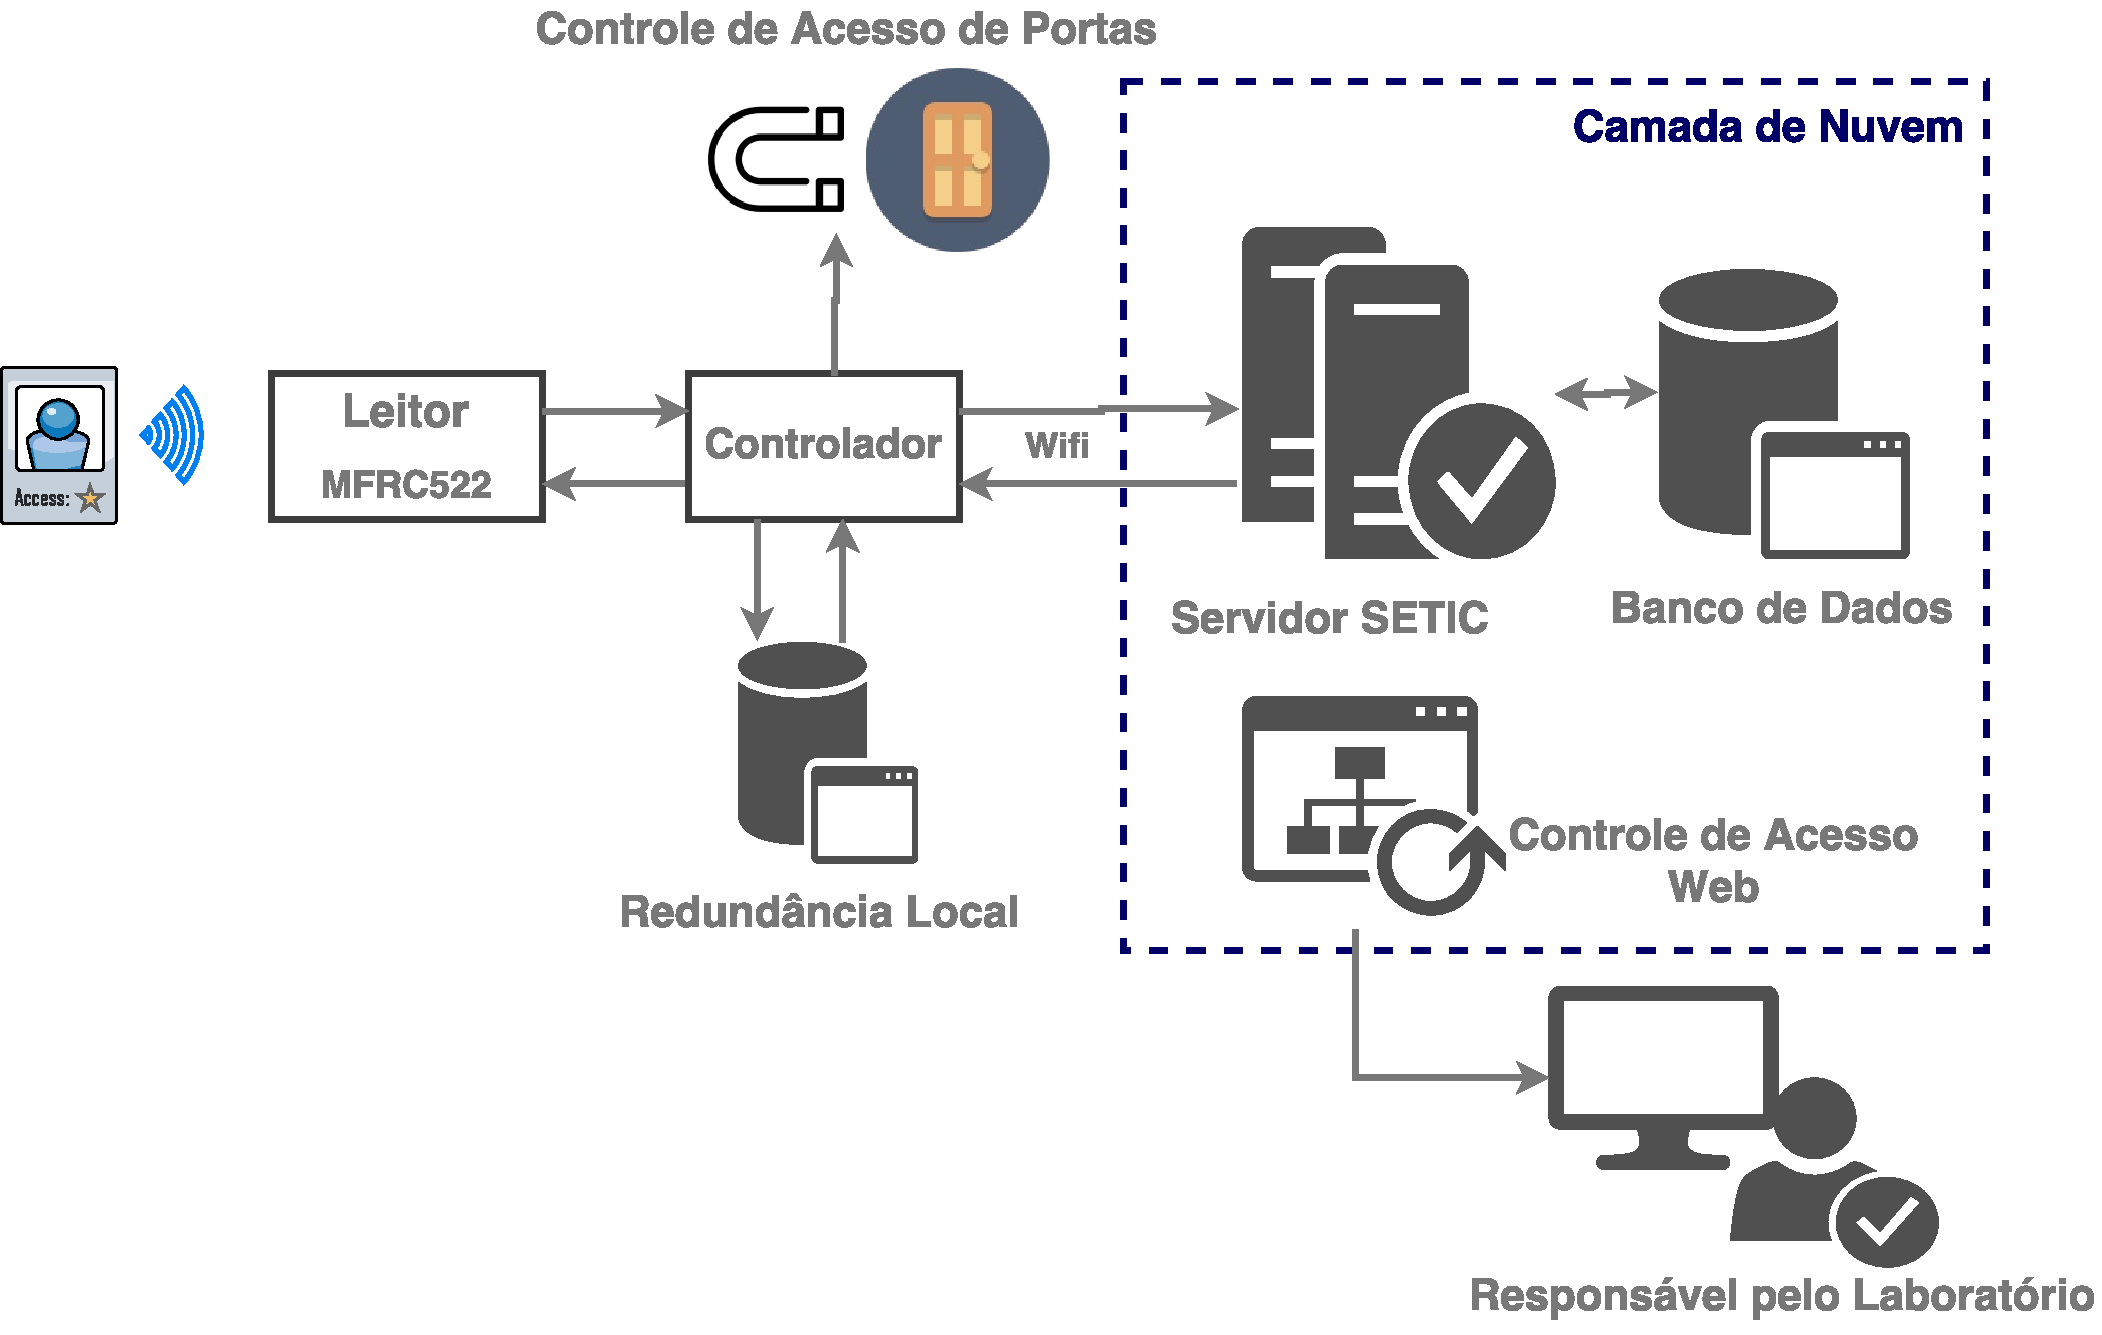
\includegraphics[width=\linewidth]{sistema}
\caption{Sistema de controle de acesso.} \label{fig:sistema}
\end{figure}

\subsection{ESP8266}

Nesse projeto, foi utilizado um módulo Nodemcu por ser um modelo de ESP8266 mais avançada, possuir maior armazenamento interno e ter melhor conectividade com o computador, além de diversas portas disponíveis.


\subsubsection{Conexão com a rede eduroam}

Para conectar os módulos na rede, é necessário utilizar a última versão do SDK mantido pela Espressif. Para conexão com a eduroam (PEAP-MS-CHAPv2), é necessário que a SDK do Espressif seja no mínimo >2.0.0. No momento que está sendo escrito essa documentação, foi utilizado a versão da biblioteca Arduino 2.4.0-rc.1 commit \texttt{c730c0f}.

Pode-se executar as seguintes linhas:

\begin{lstlisting}
cd /usr/local/arduino
cd hardware
mkdir esp8266com
cd esp8266com
git clone https://github.com/esp8266/Arduino.git esp8266

cd esp8266/tools
python get.py
\end{lstlisting}

Ou usar a seguinte plataforma no platformio.ini:

\begin{lstlisting}
platform = espressif8266_stage
\end{lstlisting}

É também necessário mudar a identidade anônima que o ESP8266 usa para acessar a rede. Não tenho certeza quanto a verdadeira necessidade dessa mudança, mas a versão de testes que conectou-se à rede utilizava a versão modificada da biblioteca libwpa2.a, da SDK do Espressif. Para modificar esse arquivo, basta localizá-lo dentro da biblioteca instalada (\path{/usr/local/arduino/hardware/esp8266com/esp8266/tools/sdk/lib} para o Arduino e  para Platformio \path{~/.platformio/packages/framework-arduinoespressif8266/tools/sdk/lib}) e executar os comandos:

\begin{lstlisting}
cp libwpa2.a libwpa2.a.bk
bbe -e "s/anonymous@espressif.com/anonymous123456@ufsc.br/" -o libwpa2.a libwpa2.a.bk
\end{lstlisting}

\subsubsection{Lista de Comandos AT}

O ESP8266 foi programado para responder a comandos do tipo AT. Para enviar um comando, deve-se enviar \texttt{AT+COMANDO}, e para passar um parâmetro, \texttt{AT+COMANDO=PARAMETRO}. Todos os comandos devem ser terminados com um carriage return (\\r). A resposta é sempre do tipo \texttt{OK} ou \texttt{ERROR}, seguida de uma descrição ou valor adicional. Exemplo:

\begin{verbatim}
AT+SYSTEMREADY\r
>OK\r
AT+GETFORMATTEDIP\r
>OK=192.168.0.25\r
AT+TIMESTAMP\r
>ERROR=CLOCKNOTSYNCED\r
\end{verbatim}

A Tabela \ref{tabela-comandos} mostra os comandos disponíveis para o ESP8266.

\begin{table}[!ht]
\centering
\caption{Tabela de Comandos do firmware do ESP8266}
\vspace{0.5cm}
\label{tabela-comandos}
\renewcommand*{\arraystretch}{1.7}
\begin{tabularx}{\linewidth}{|X|X|}
\hline
\textbf{Comando} & \textbf{Retorno} \\
\hline
\textbf{AT+SYSTEMREADY} & Retorna se o filesystem e a conexão WiFi estão funcionais. \\ \hline
\textbf{AT+CONNECTWIFI} & Tenta se conectar ao WiFi padrão do firmware (executado por padrão no início). \\ \hline
\textbf{AT+TIMESTAMP} & Retorna a string de um inteiro de 32 bits representando o Epoch time. \\ \hline
\textbf{AT+FTIMESTAMP} & Retorna o timestamp completo formatado segundo a norma ISO 8601. \\ \hline
\textbf{AT+HEAPSIZE} & Retorna o tamanho da memória heap do ESP8266. \\ \hline
\textbf{AT+GET=url}    & Envia uma requisição do tipo HTTP GET para a url e retorna o conteúdo sem os headers. \\ \hline
\textbf{AT+GETS=url}    & Envia uma requisição do tipo HTTPS GET para a url e retorna o conteúdo sem os headers. \\ \hline
\textbf{AT+PAYLOAD=payload}    & Cria um payload para requisições do tipo POST, e é consumido após chamar o comando POST. \\ \hline
\textbf{AT+POST=url}    & Envia uma requisição do tipo HTTP POST para a url com o conteúdo do PAYLOAD e retorna o conteúdo sem os headers. \\ \hline
\textbf{AT+POSTS=url}    & Envia uma requisição do tipo HTTPS POST para a url com o conteúdo do PAYLOAD e retorna o conteúdo sem os headers. \\ \hline
\textbf{AT+IP}       & Retorna a string de um inteiro de 32 bits representando o IP do nodo. \\ \hline
\textbf{AT+FIP} & Retorna o IP formatado do nodo. \\ \hline
\textbf{AT+RSSI} & Retorna o RSSI do wifi\_station. \\ \hline
\textbf{AT+CHANNEL} & Retorna o canal do Wifi. \\
\hline
\end{tabularx}
\end{table}


\subsection{EPOS Mote III}

Para implementação no nodo EPOS, existem três elementos básicos, a ligação e comunicação com o módulo ESP8266, a ligação com o módulo MFRC522 e a ligação com relé da Hydro Board.

Para fazer todo o protótipo funcionar foi necessário utilizar uma versão modificada da classe do EPOS \texttt{Persistent\_Ring\_FIFO}, e foi criada uma nova classe chamada \texttt{Persistent\_Ring} que resolve esse problema, tendo tanto funções \texttt{pop\_fifo()} como \texttt{pop\_filo()}.

O modo de funcionamento do EPOS nesse cenário pode ser visto na \figurename~\ref{fig:diagrama_modulo}.

\begin{figure}[!ht]
\centering
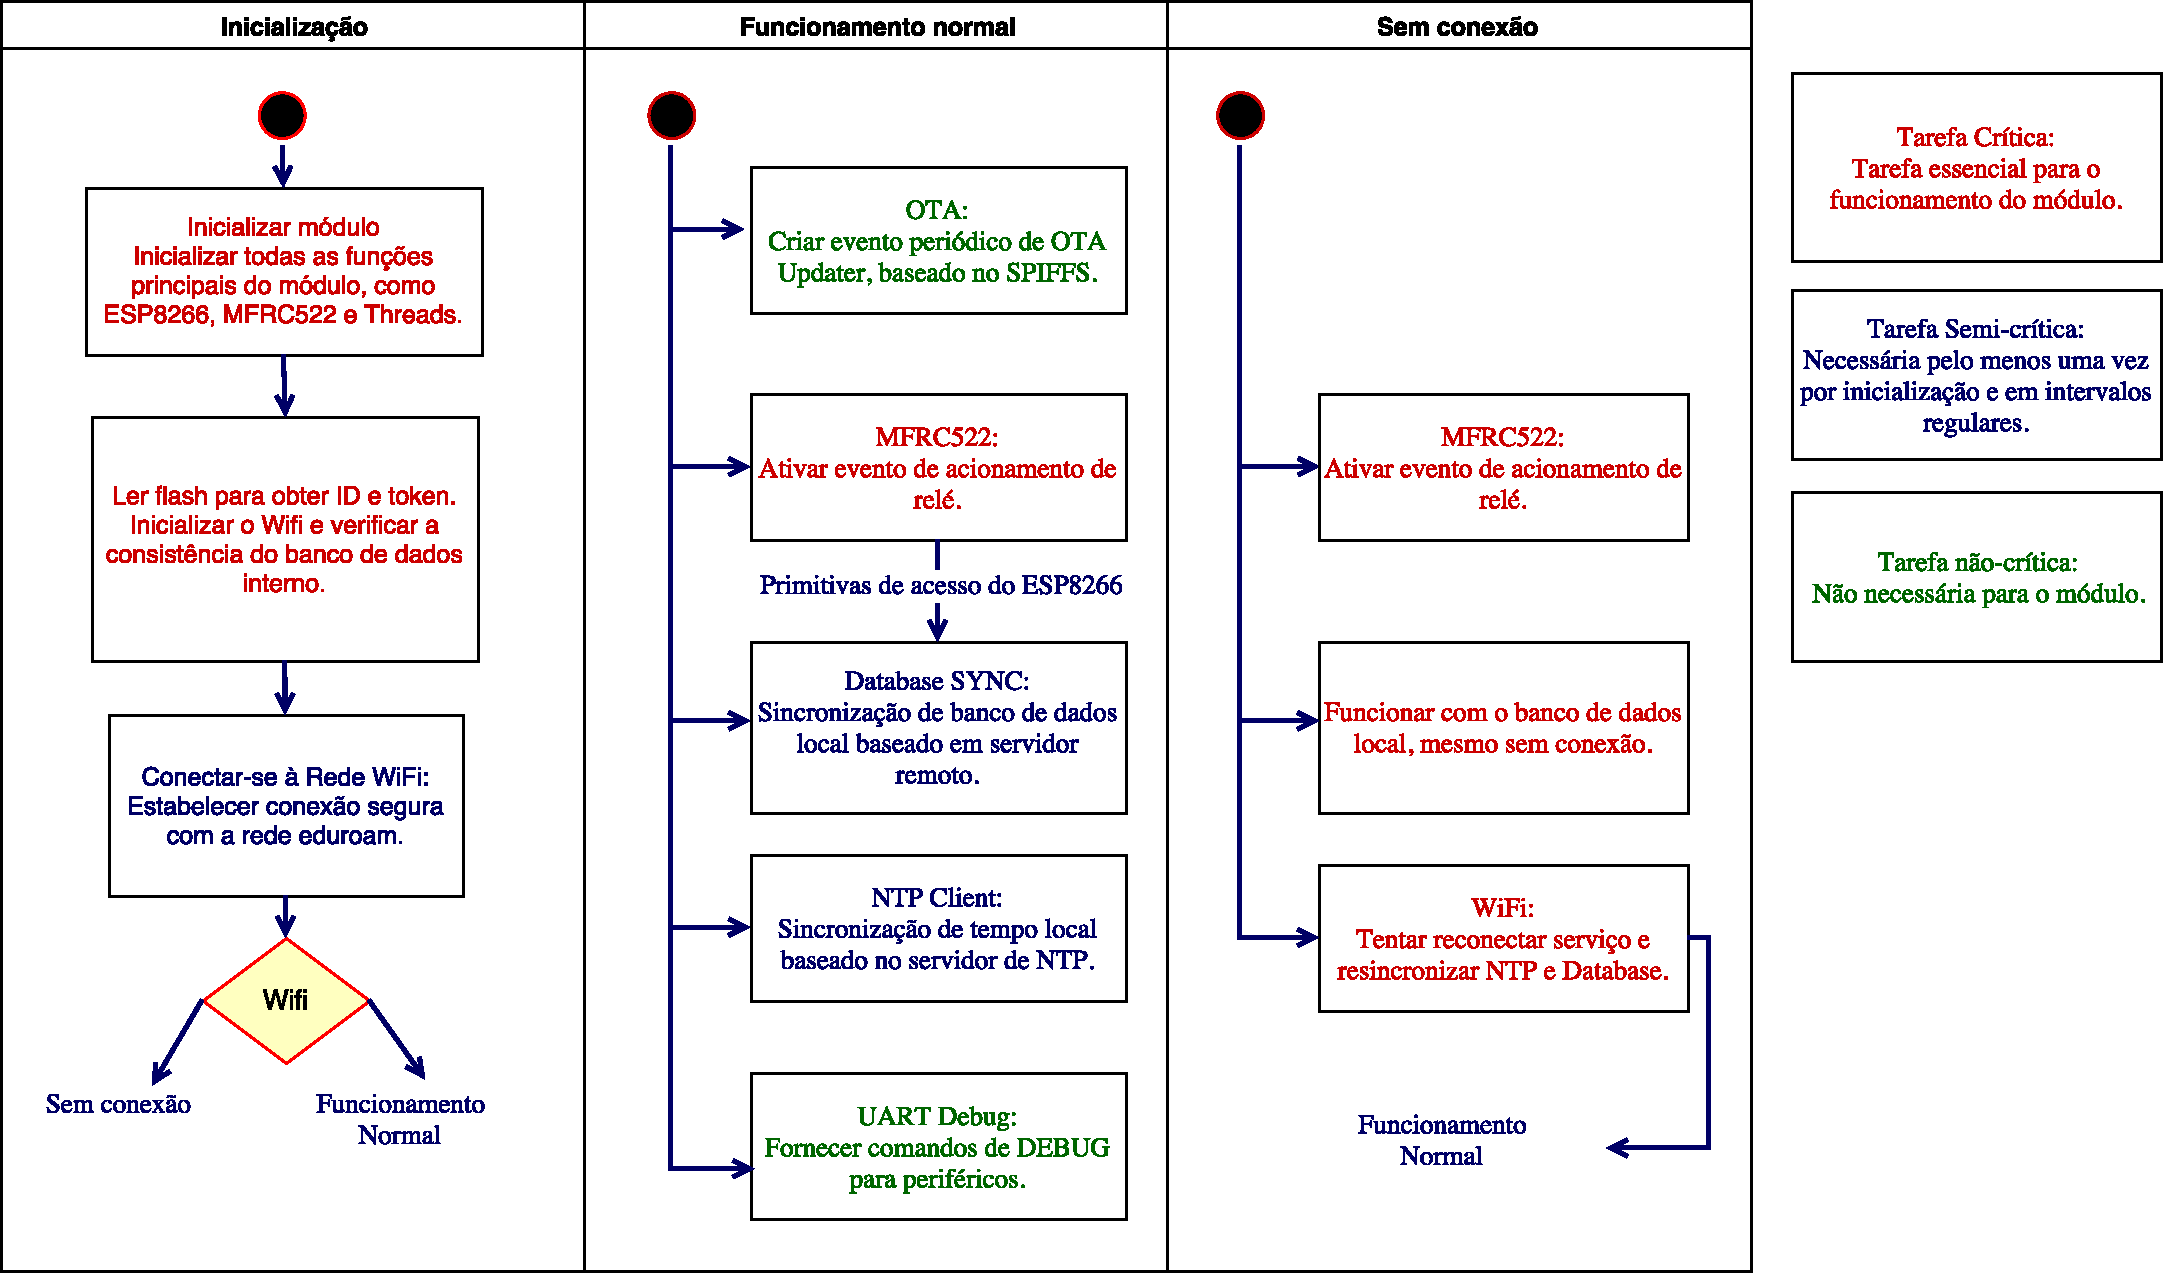
\includegraphics[width=\linewidth]{diagrama_modulo}
\caption{Diagrama de funcionamento do eMote3.} \label{fig:diagrama_modulo}
\end{figure}

\subsubsection{ESP8266}

O ESP8266 aceita os requests do EPOS do tipo serial (baud 115200) e \textbf{não é uma classe síncrona, ou seja, não trata concorrência}. Ainda não foi estudado os impactos da forma insegura de transmissão de dados via serial.

A ligação dos módulos pode ser vista na \figurename~\ref{fig:emote-esp8266}.

\begin{figure}[!ht]
\centering
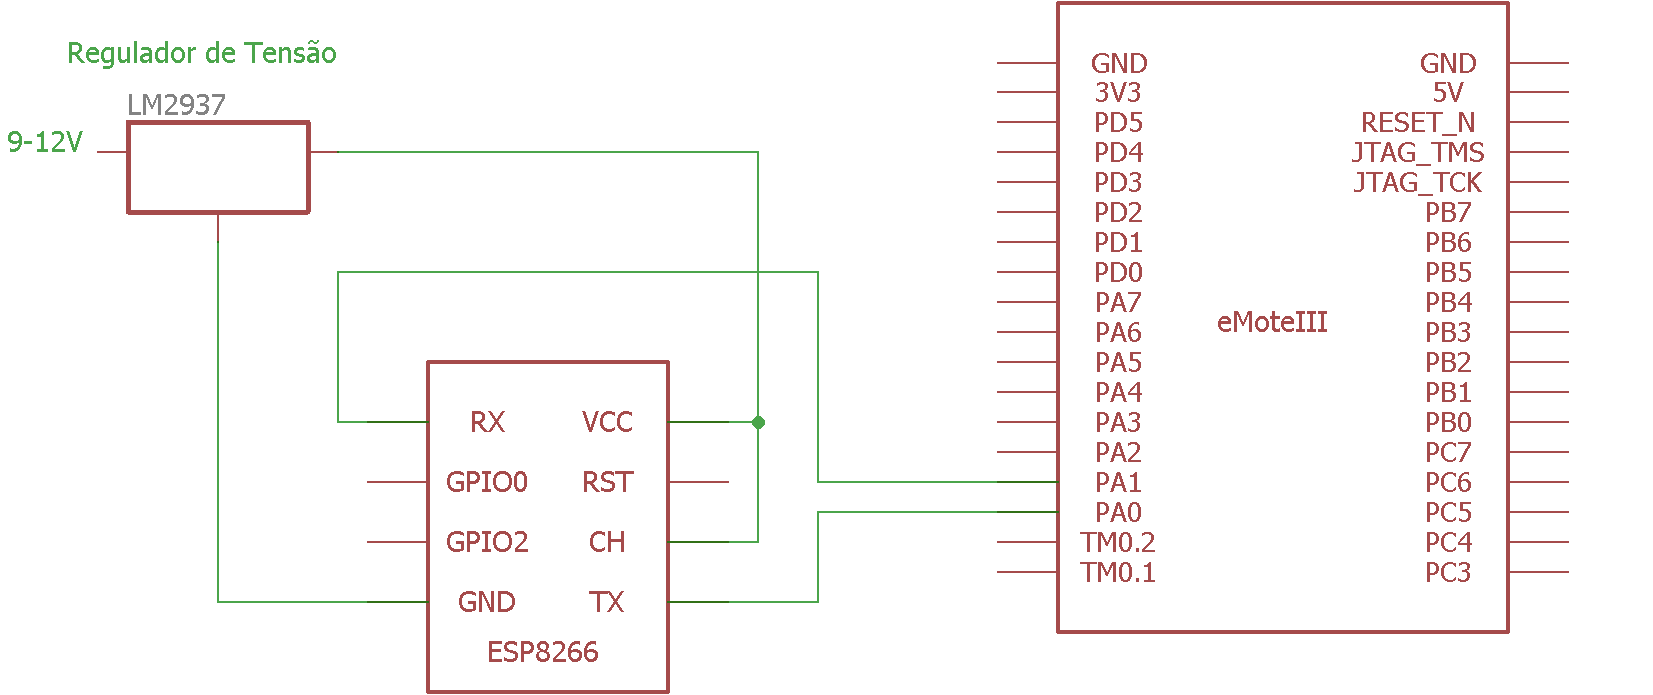
\includegraphics[width=.7\linewidth]{emote-esp8266}
\caption{Diagrama de ligação eMote3-ESP8266.} \label{fig:emote-esp8266}
\end{figure}

\subsubsection{MFRC522}

O módulo RFID MFRC522 roda em uma Thread que lê os cartões, lê o banco de dados na presença de um cartão, gera uma chamada de acesso (permitido ou negado) e despacha uma nova entrada no banco de dados local, para depois ser persistido pela rotina de sincronização.

A ligação dos módulos pode ser vista na \figurename~\ref{fig:emote-mfrc522}.

\begin{figure}[!ht]
\centering
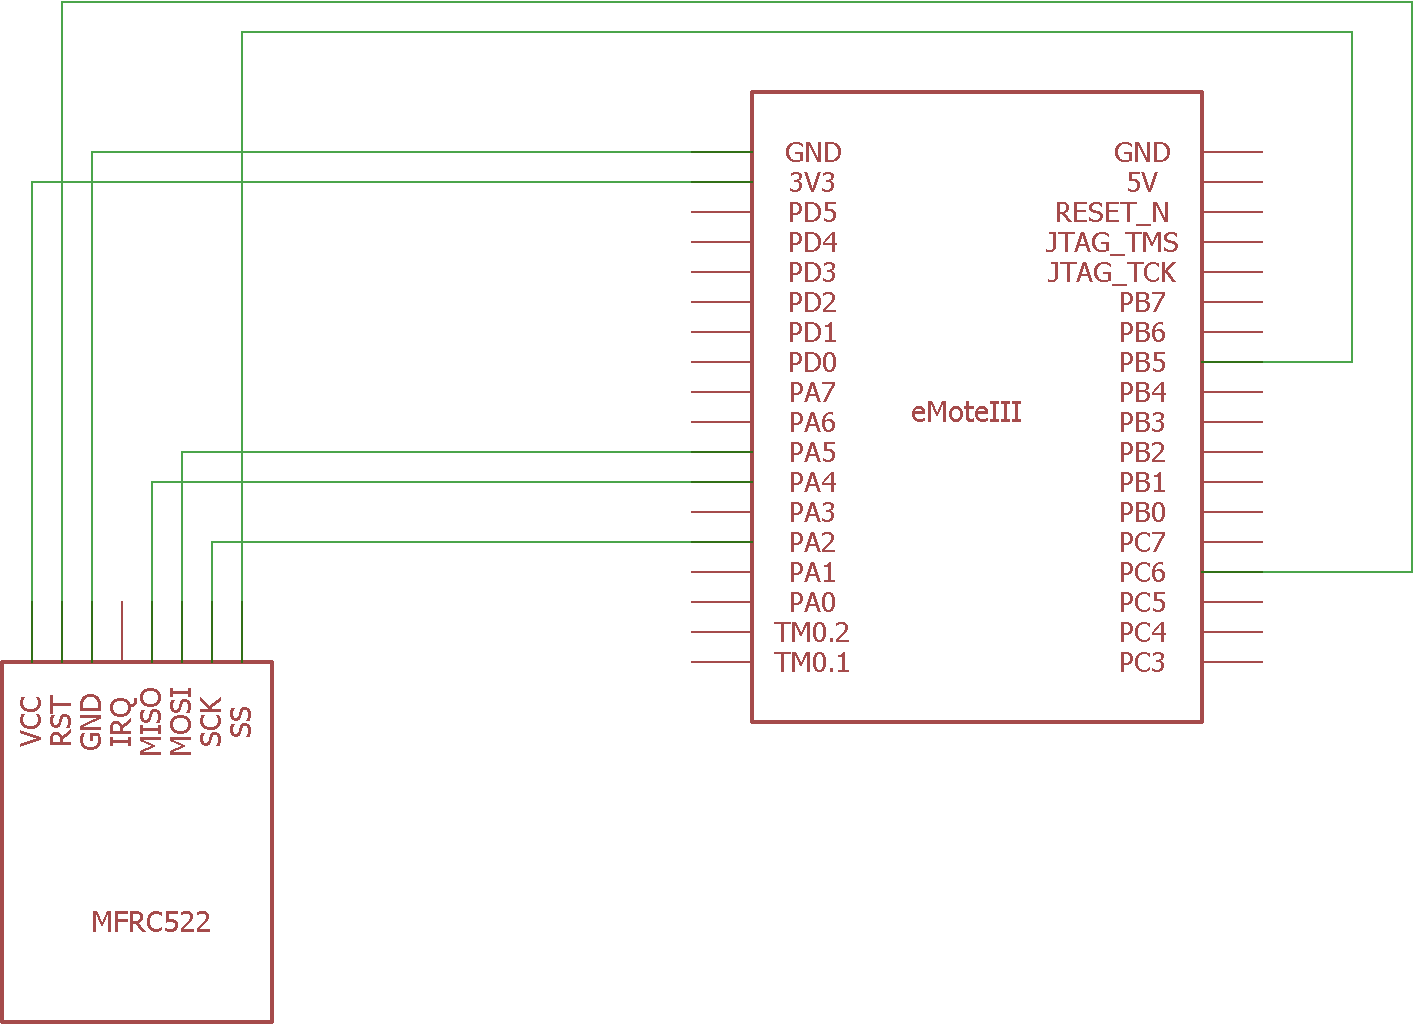
\includegraphics[width=.7\linewidth]{emote-mfrc522}
\caption{Diagrama de ligação eMote3-MFRC522.} \label{fig:emote-mfrc522}
\end{figure}

\subsubsection{Hydro Board}

A Hydro Board ainda não foi testada. Um LED está sendo usado em seu lugar para simular o relé.

\subsubsection{Banco de Dados local}

Como já dito, o banco de dados local foi implementado em \texttt{Persistent\_Ring}. Seria preferível implementá-lo utilizando o sistema de RIFFS (filesystem) que está sendo produzido para o EPOS, mas ele se mostrou instável e com funções faltantes, e era muito complexo para ser adaptado ao cenário.

Para isso, foi implementado um sistema de armazenamento interno, que respeita a seguinte lógica de funcionamento:

\begin{enumerate}
\item Um evento é chamado em uma função \texttt{rfid\_reader()}, empurrando uma nova entrada no armazenamento interno.
\item A função de manutenção do banco de dados roda em intervalos específicos, utilizando a classe \texttt{Periodic\_Thread} do EPOS.
\item Quando a função de manutenção é acordada, ela realiza dois passos em ordem:
\begin{enumerate}
\item Persistir todas as entradas de dados na nuvem, que possuem nível de importância maior.
\item Atualizar o banco de dados interno com a relação de UIDs que tem acesso à sala.
\end{enumerate}
\item Caso o acesso ao meio esteja comprometido e o nodo não consiga atualizar-se com a nuvem, ele espera novamente o tempo de ciclo e volta ao passo 3.
\end{enumerate}

\subsubsection{Instalando o firmware no dispositivo}

O dispositivo ainda não conta com uma build automatizada. Logo, para fazer sua própria build, siga os seguintes passos:

\begin{lstlisting}
cd arm/
# alterar o id e o token no codigo em app/rfid_door_blumenau.cc
make APPLICATION=rfid_door_blumenau flash
# conectar o EPOS Mote
# fazer as conexoes fisicas
\end{lstlisting}

\end{document}
